\subsection{Subsystem Decomposition}
\begin{figure}[H]
	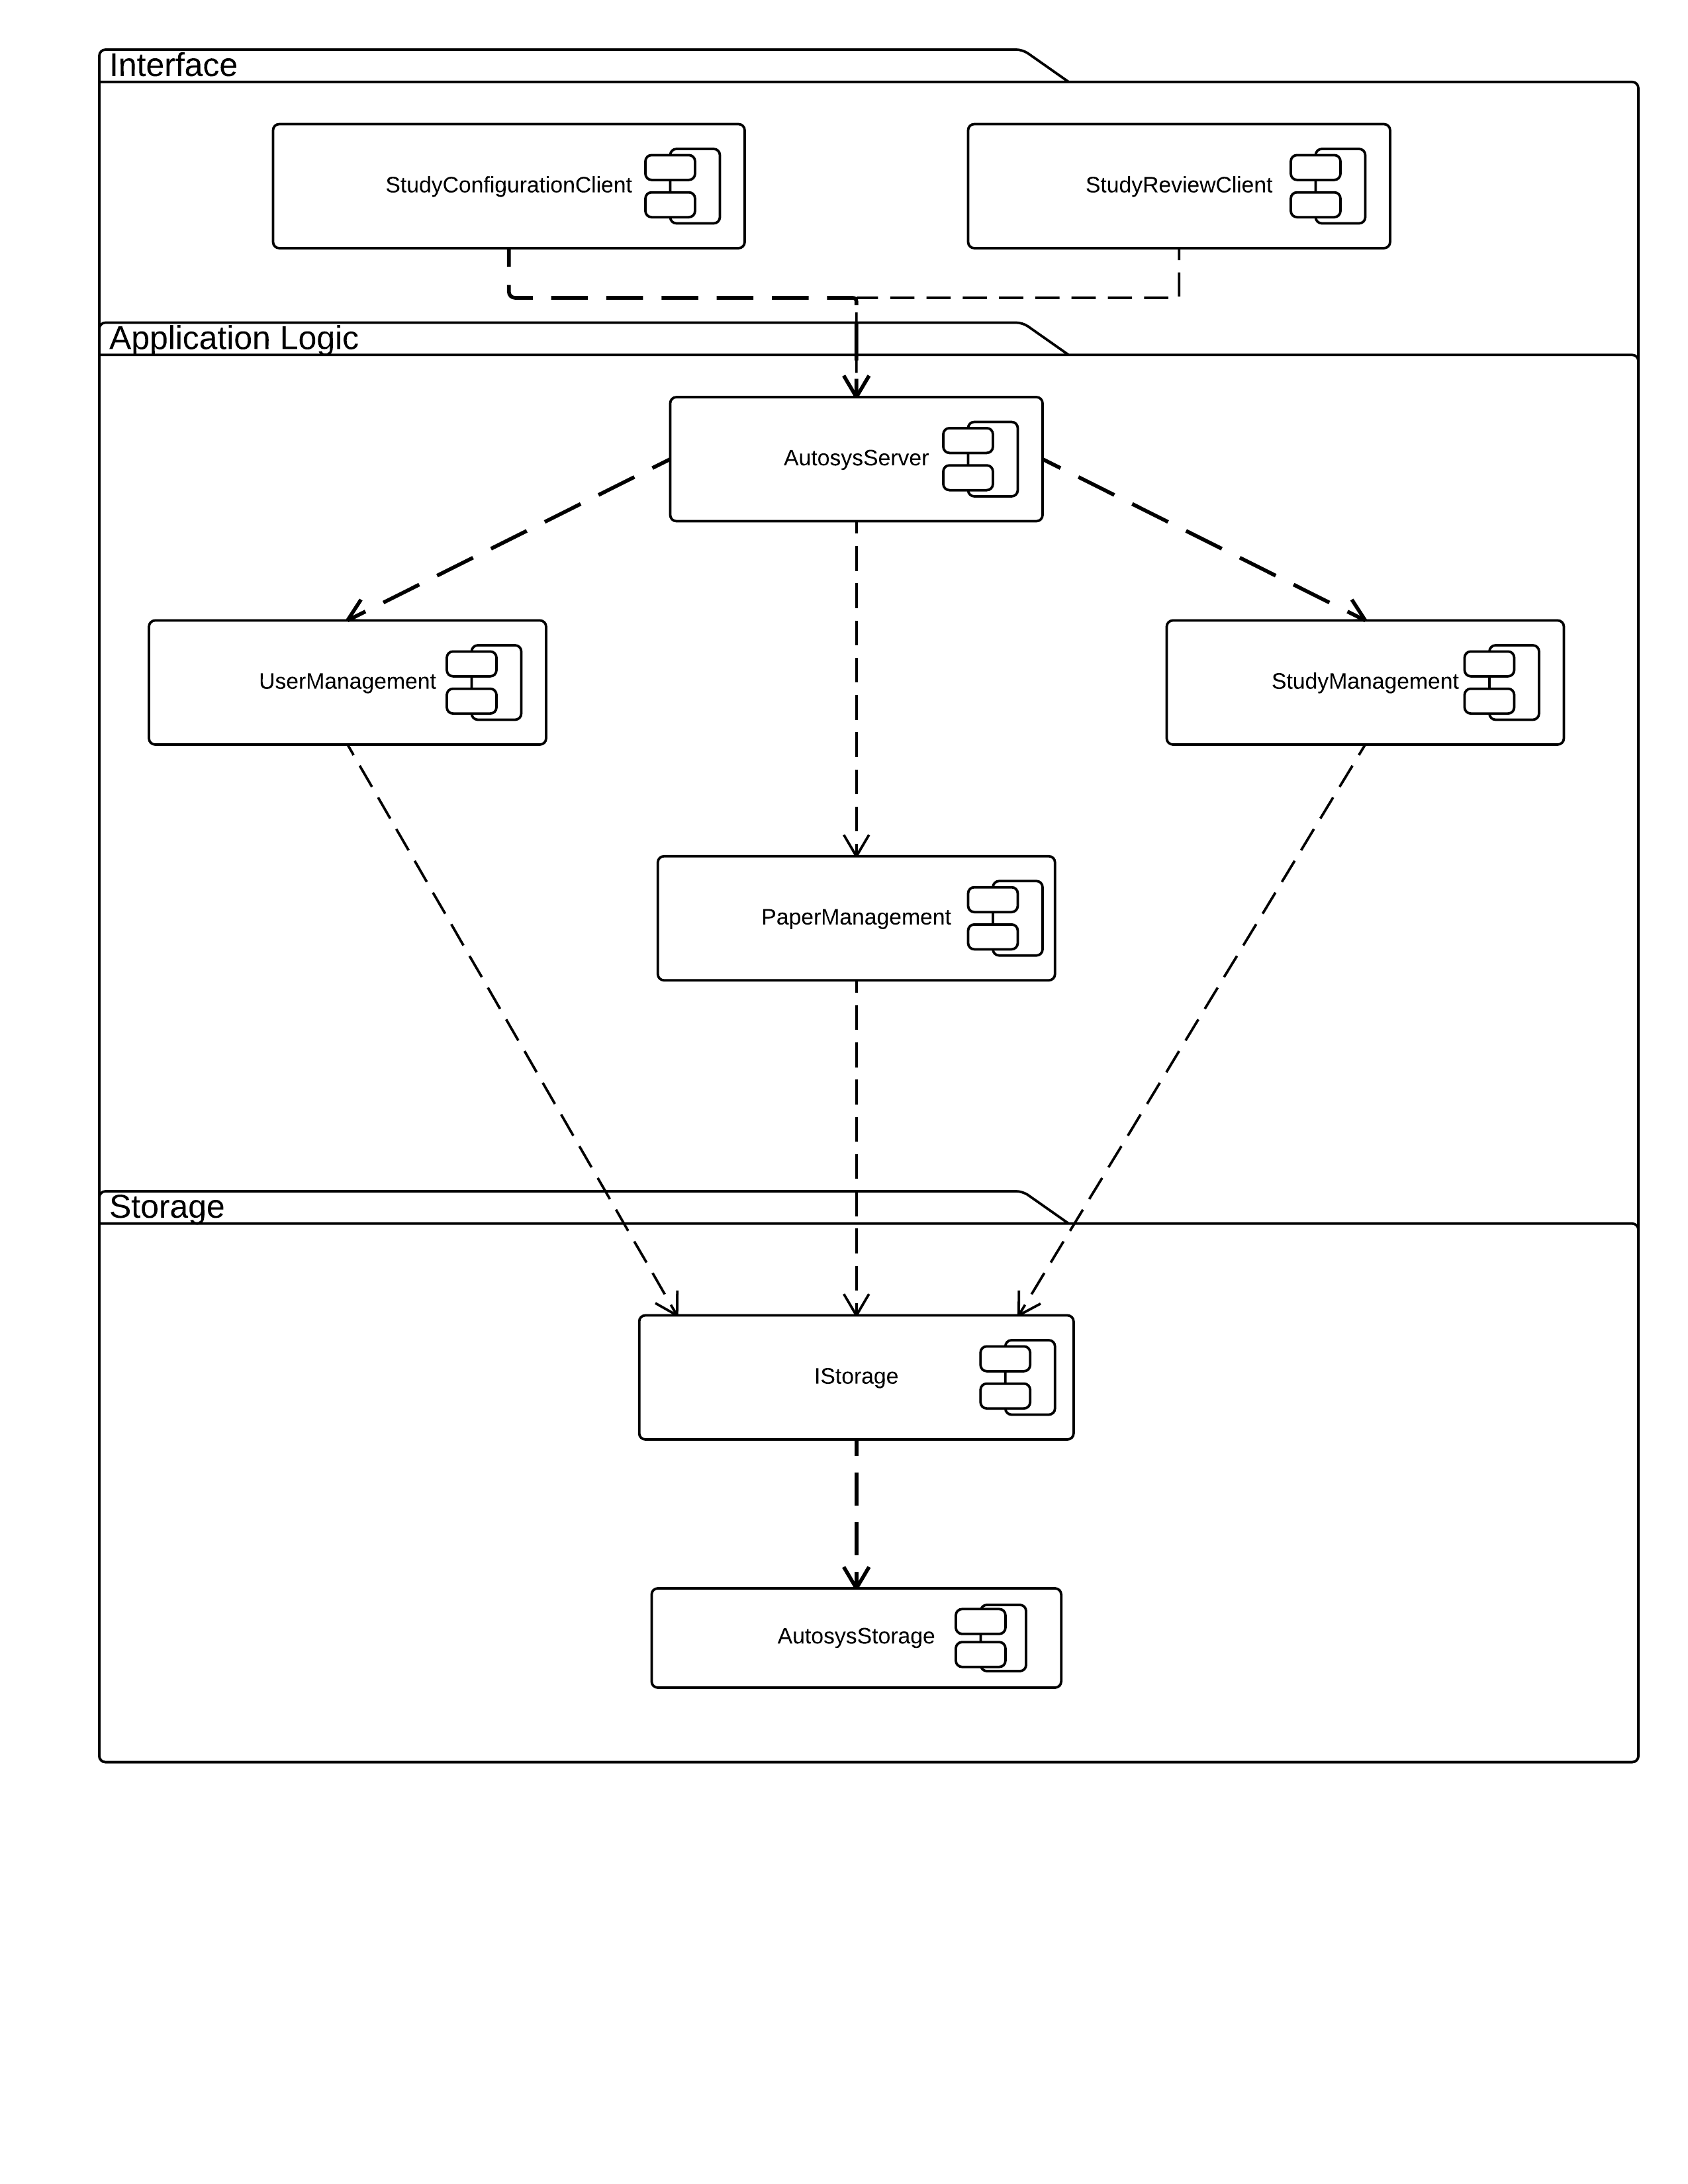
\includegraphics[width = \linewidth]{subsections/UMLComponentDiagramSubsystems}
	\caption{Autosys subsystem decomposition (UML Component Diagram, layers shown as UML packages)}
	\label{fig:Subsystem Decomposition, UML Component Diagram}
\end{figure}
The subsystems are identified from the functional requirements of the Autosys RAD document. A three-tier architectural style has been used for the decomposition of the system where a \textbf{StudyConfigurationClient} provides a front end for users to initiate all use cases related to setting up or configuring a \textbf{Study}. Also a \textbf{StudyReviewClient} will provide the front end for users to manage teams, and work with review tasks.
The \textbf{AutosysServer} will be managing access control, concurrency control, and delegates to nested subsystems for the application logic. The \textbf{UserManagement} component is holding the responsibility for handling all CRUD operations regarding teams and individual users. The processing of all Study related CRUD operations are carried out by the \textbf{StudyManagement} component. The  \textbf{StudyManagement} also manages Study Tasks, Study Criteria and Classifications, Study Phases and he other parts included in a study. The \textbf{PaperManagement} runs the filtering mechanisms on the research papers and does import/export of research papers according to the Study Criteria and Classifications.
The\textbf{ IStorage} interface is used for a Bridge Pattern to decouple the storage abstraction from the application logic so that the two can vary independently. At the bottom tier the \textbf{AutosysStorage} represents the subsystem for storing the user data, study data, and research papers.